\input{preamble.tex}
\newcommand{\C}{\mathcal{C}}
\pgfplotsset{tick style={very thin}} 


\begin{document}
\pagestyle{fancy}
\fancyhead[L]{Seconde}
\fancyhead[C]{\textbf{Evaluation flash n°4a}}
\fancyhead[R]{\today}

\reversemarginpar

\null\vspace{-30pt}
Nom / Prénom : \\

Consignes particulières : 
\begin{itemize}[label=$\bullet$]
	\item 
	La calculatrice est \textbf{interdite}.
%	\item 
%	Le devoir peut être fait entièrement sur cette feuille.
%	\item 
%	Toute trace de recherche est prise en compte.
	%\item 
	%L'abbréviation $\tq$ signifie ``tel que''.
\end{itemize}

\hrule

\exe{4}{
Pour chacune des paires de points $A$, $B$ suivantes, calculer les paramètres ($a$ et $b$) de
l’unique fonction affine $f$ telle que $A$ et $B$ appartiennent à $\C_f$ .
\begin{enumerate}
\item $A(1;-2)$ et $B(5;0)$ ;
\item $A(-3;2)$ et $B(-5;4)$
\end{enumerate}
}{exe:1a}{
\begin{enumerate}
\item $a=\dfrac12$ et $b=-\dfrac52$ ;
\item $a=-1$ et $b=-1$.
\end{enumerate}
}

\exe{6}{
On considère la fonction $f$ d'expression algébrique $f(x) = \dfrac14 x - 2$.
\begin{enumerate}
\item Donner les paramètres $a$ et $b$ de cette fonction affine.
\item Tracer la courbe de $f$ dans un repère orthonormé.
\item Le point $P(8;0)$ appartient-il à $\C_f$ ? Justifier.
\item On considère maintenant la fonction $g$ passant par les points $A(0;2)$ et $B(1;0)$.
\begin{enumerate}
\item Déterminer l'expression algébrique de $g$.
\item Représenter $g$ dans le repère précédent.
\item Déterminer $x$ tel que $f(x)=g(x)$.
\end{enumerate}
\end{enumerate}
}{exe:2a}{
\begin{enumerate}
\item $a=\dfrac14$ et $b=-2$.
\item 
	\begin{center}
	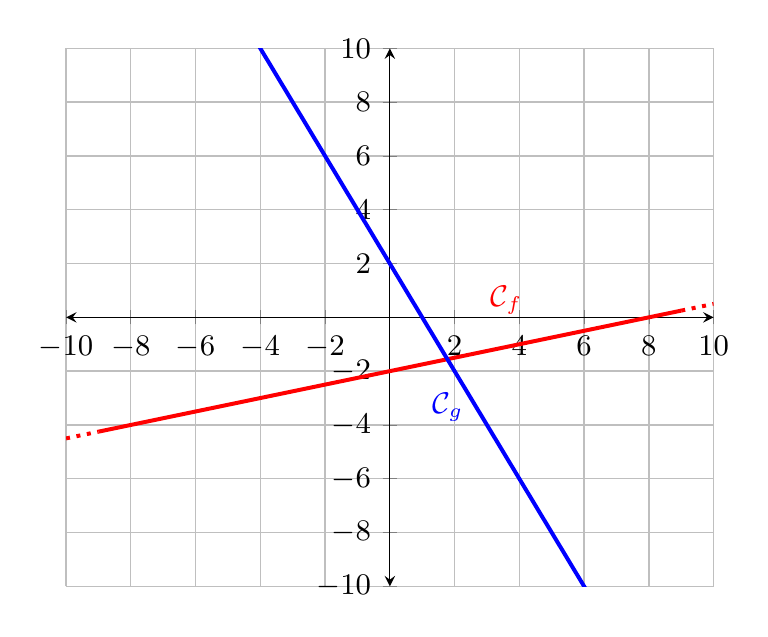
\begin{tikzpicture}[>=stealth, scale=1.2, every node/.append style={font=\small}]
	\begin{axis}[xmin = -10, xmax=10, ymin=-10, ymax=10, axis x line=middle, axis y line=middle, axis line style=<->, xlabel={}, ylabel={}, xtick = {-10, -8, ..., 8, 10}, ytick = {-10, -8, ..., 8, 10}, grid=both]
	
		\addplot[red, very thick, domain =-9:9, samples=2] {x/4-2}  node[pos=.7, above=6pt] {$\mathcal{C}_f$};
		\addplot[red, very thick, dotted, domain =-10:-9, samples=2] {x/4-2} ;
		\addplot[red, very thick, dotted, domain =9:10, samples=2] {x/4-2};
	
	
		\addplot[blue, very thick, domain =-9:9, samples=2] {-2*x+2}  node[pos=.6, below=6pt] {$\mathcal{C}_g$};
		\addplot[blue, very thick, dotted, domain =-10:-9, samples=2] {-2*x+2} ;
		\addplot[blue, very thick, dotted, domain =9:10, samples=2] {-2*x+2};
	\end{axis}
	\end{tikzpicture}
	\end{center}
\item Par calcul : $f(8)=\dfrac14 \times 8 -2 = 2 - 2 = 0$, donc oui.
\item 
\begin{enumerate}
\item $g(x)=-2x+2$
\item Voir question 2.
\item On cherche $x$ tel que $\dfrac14 x - 2 = -2x+2$ soit $\dfrac94 x = 4$ donc $x=\dfrac{16}9$.
\end{enumerate}
\end{enumerate}

}

\newpage

\setcounter{Exercise}{0}

\pagestyle{fancy}
\fancyhead[L]{Seconde}
\fancyhead[C]{\textbf{Evaluation flash n°4b}}
\fancyhead[R]{\today}

\reversemarginpar

\null\vspace{-30pt}
Nom / Prénom : \\

Consignes particulières : 
\begin{itemize}[label=$\bullet$]
	\item 
	La calculatrice est \textbf{interdite}.
%	\item 
%	Le devoir peut être fait entièrement sur cette feuille.
%	\item 
%	Toute trace de recherche est prise en compte.
	%\item 
	%L'abbréviation $\tq$ signifie ``tel que''.
\end{itemize}

\hrule

\exe{}{
Pour chacune des paires de points $A$, $B$ suivantes, calculer les paramètres ($a$ et $b$) de
l’unique fonction affine $f$ telle que $A$ et $B$ appartiennent à $\C_f$ .
\begin{enumerate}
\item $A(1;3)$ et $B(5;1)$ ;
\item $A(-3;2)$ et $B(-6;-4)$
\end{enumerate}
}{exe:1b}{
\begin{enumerate}
\item $a=-\dfrac12$ et $b=\dfrac72$ ;
\item $a=2$ et $b=8$.
\end{enumerate}
}

\exe{}{
On considère la fonction $f$ d'expression algébrique $f(x) = -\dfrac13 x + 4$.
\begin{enumerate}
\item Donner les paramètres $a$ et $b$ de cette fonction affine.
\item Tracer la courbe de $f$ dans un repère orthonormé.
\item Le point $P(9;1)$ appartient-il à $\C_f$ ? Justifier.
\item On considère maintenant la fonction $g$ passant par les points $A(0;1)$ et $B(1;3)$.
\begin{enumerate}
\item Déterminer l'expression algébrique de $g$.
\item Représenter $g$ dans le repère précédent.
\item Déterminer $x$ tel que $f(x)=g(x)$.
\end{enumerate}
\end{enumerate}
}{exe:2b}{
\begin{enumerate}
\item $a=-\dfrac13$ et $b=4$.
\item 
	\begin{center}
	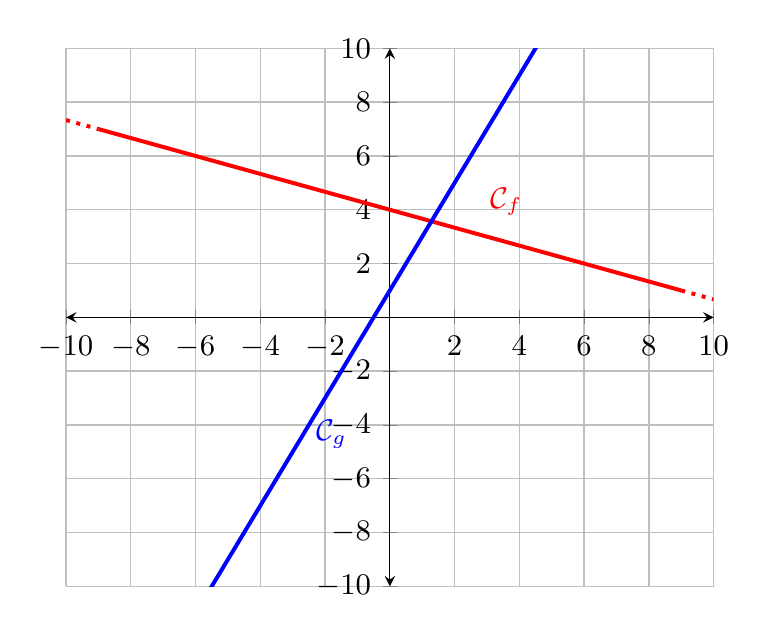
\begin{tikzpicture}[>=stealth, scale=1.2, every node/.append style={font=\small}]
	\begin{axis}[xmin = -10, xmax=10, ymin=-10, ymax=10, axis x line=middle, axis y line=middle, axis line style=<->, xlabel={}, ylabel={}, xtick = {-10, -8, ..., 8, 10}, ytick = {-10, -8, ..., 8, 10}, grid=both]
	
		\addplot[red, very thick, domain =-9:9, samples=2] {-x/3+4}  node[pos=.7, above=4pt] {$\mathcal{C}_f$};
		\addplot[red, very thick, dotted, domain =-10:-9, samples=2] {-x/3+4} ;
		\addplot[red, very thick, dotted, domain =9:10, samples=2] {-x/3+4};
	
	
		\addplot[blue, very thick, domain =-9:9, samples=2] {2*x+1}  node[pos=.4, below=6pt] {$\mathcal{C}_g$};
		\addplot[blue, very thick, dotted, domain =-10:-9, samples=2] {2*x+1} ;
		\addplot[blue, very thick, dotted, domain =9:10, samples=2] {2*x+1};
	\end{axis}
	\end{tikzpicture}
	\end{center}
\item Par calcul : $f(9)=-\dfrac13 \times 9 + 4 = -3 + 4 = 1$, donc oui.
\item 
\begin{enumerate}
\item $g(x)=2x+1$
\item Voir question 2.
\item On cherche $x$ tel que $-\dfrac13 x + 4 = 2x+1$ soit $\dfrac73 x = 3$ donc $x=\dfrac97$.
\end{enumerate}
\end{enumerate}

}


%%%%%%%%%%%%

\newpage
\fancyhead[C]{\textbf{Solutions}}
\shipoutAnswer

\end{document}
 